In this section, we show empirical results of our algorithm on different transferring situations on two datasets: AwA10\footnote{The features of AwA dataset is available from http://attributes.kyb.tuebingen.mpg.de/} \cite{lampert2009learning} and Caltech10\footnote{Images for Caltech is available from http://www.vision.caltech.edu/Image\_Datasets/Caltech256/} \cite{griffin2007caltech}. In real world applications, there are three situations in HTL. The first two extreme cases are all the hypotheses are correct/incorrect. The third one is the intermediate (mixed) case where only part of the hypotheses are correct. We design three sets of experiment, called positive, negative and mixed transfer experiment respectively, based on these 3 situations, comparing our algorithm with the baselines.
\subsection{Dataset}
Caltch10 is a subset of Caltech256. We select the following 10 categories: \textit{bat, bear, dolphin, giraffe, gorilla, horse, leopard, raccoon, skunk, zebra}, containing 1387 images, as our dataset.
AwA10 is a subset of AwA dataset. We choose the identical 10 categories as those in Caltech10 from it, containing 6917 images.

\subsection{Baselines and algorithmic setup}
We compare our algorithm with two kinds of baselines. The first one is methods without leveraging any prior knowledge (no transfer baselines). The second consists of some methods with transfer techniques. 

We select 3 no transfer baselines:
\textbf{No transfer:} LS-SVM trained only on target data. Any transfer algorithm that performs worse than it suffers from negative transfer. \textbf{Batch:} We combined the source and target data, assuming that we have full access to all data, to train the LS-SVM. The result of this baseline might be considered as the best performance achieved when the hypotheses are correct. We only perform this baseline in positive transfer experiment. \textbf{Source+1:} This method only train a new binary LS-SVM for the new category. For the rest of the classes, we use the predictions of the classifiers trained from source data directly. Its performance indicates the correctness of the hypotheses.


We select the 3 HTL methods, {MKTL \cite{jie2011multiclass}}, {MULTI-KT \cite{tommasi2014learning}} and MULTIpLE \cite{kuzborskij2013n}, as our transfer baselines.

%\textbf{MKTL \cite{jie2011multiclass}:} This method uses the output of source models as extra feature inputs and automatically determine from which source models to transfer and how much to transfer.


%\textbf{MULTI-KT \cite{tommasi2014learning}:} This method has similar idea with MKTL. It uses LOO error to determine how much to transfer from source models and convert it into solving the convex optimization problem.

%\textbf{MULTIpLE \cite{kuzborskij2013n}:} The basic setting of this method is similar to ours. It is designed to balance the performance between learning the new category and preserving the model from prior knowledge.

For all the experiments in this section, we adopt the same strategy as \cite{kuzborskij2013n} and \cite{tommasi2014learning}, using kernel averaging \cite{gehler2009feature} to compute the average of RBF kernels over the available features on RBF hyperparameter $\{2^{-5},2^{-4},...,2^8\}$. The penalty parameter $C$ is tuned via cross-validation on $\{10^{-5},10^{-4},...,10^8\}$ and the optimal value is reused for all the algorithms.
Two transfer regularization parameters $\lambda1$ and $\lambda2$ are also set via cross-validation on $\{10^{-3},10^{-2},...,10\}$ respectively.

\subsection{Positive transfer: transferring from correct hypotheses}
In the extreme case, where the hypotheses are correct, the data of the source and target tasks should be drawn from the same distribution. Thus, we perform two experiments under this setting on both AwA and Caltech. For each dataset, we split the data into two sets. One is treated as the source dataset to train the source hypotheses and another is treated as the target dataset for training and testing. We iteratively choose one category as the new category and run the experiment 10 times. Due to space constraint, we only report the average results of the two experiments in Table \ref{tab:C2C} and Table \ref{tab:A2A}. From the results, we can see that SMITLe can achieve high classification accuracy than other baselines in most of the cases.
%in Caltech experiment, our algorithm consistently outperforms all the baselines (even better than Batch method). In AwA dataset, Source+1 outperforms SMITLe when the training size is 5. As we increase the training size, the accuracy of SMITLe increases and outperforms Source+1.

To illustrate the detail performance of our algorithm, we select the experiment result on AwA dataset where the horse is chosen as the new category for further explanation. %In Figure \ref{fig:awa-a}, we show the average performances of different methods on different training size for 10 experiments. We can observe that, as the training size increases, our method can even outperform the batch method.
In Figure \ref{fig:awa} we provide values of $\gamma$ and $\beta$ compared with the parameters of the runner-up transfer algorithm MULTIpLE. We can see that for transfer knowledge between identical categories, MULTIpLE fixes the transfer parameter ($\gamma$) to be 1 while our method sets greater weights for related prior knowledge. By exploiting the positive prior knowledge more aggressively, SMITLe is able to leverage the prior knowledge and outperforms other methods. For the transfer parameter $\beta$ we can see that MULTIpLE tends to keep $\beta$ greater than 0 and SMITLe works more intuitively, setting the positive weight for related categories(giraffe, zebra, and bear etc.) and small or even negative weight for unrelated categories (bat, dolphin, and skunk etc.).


\begin{figure}
\centering
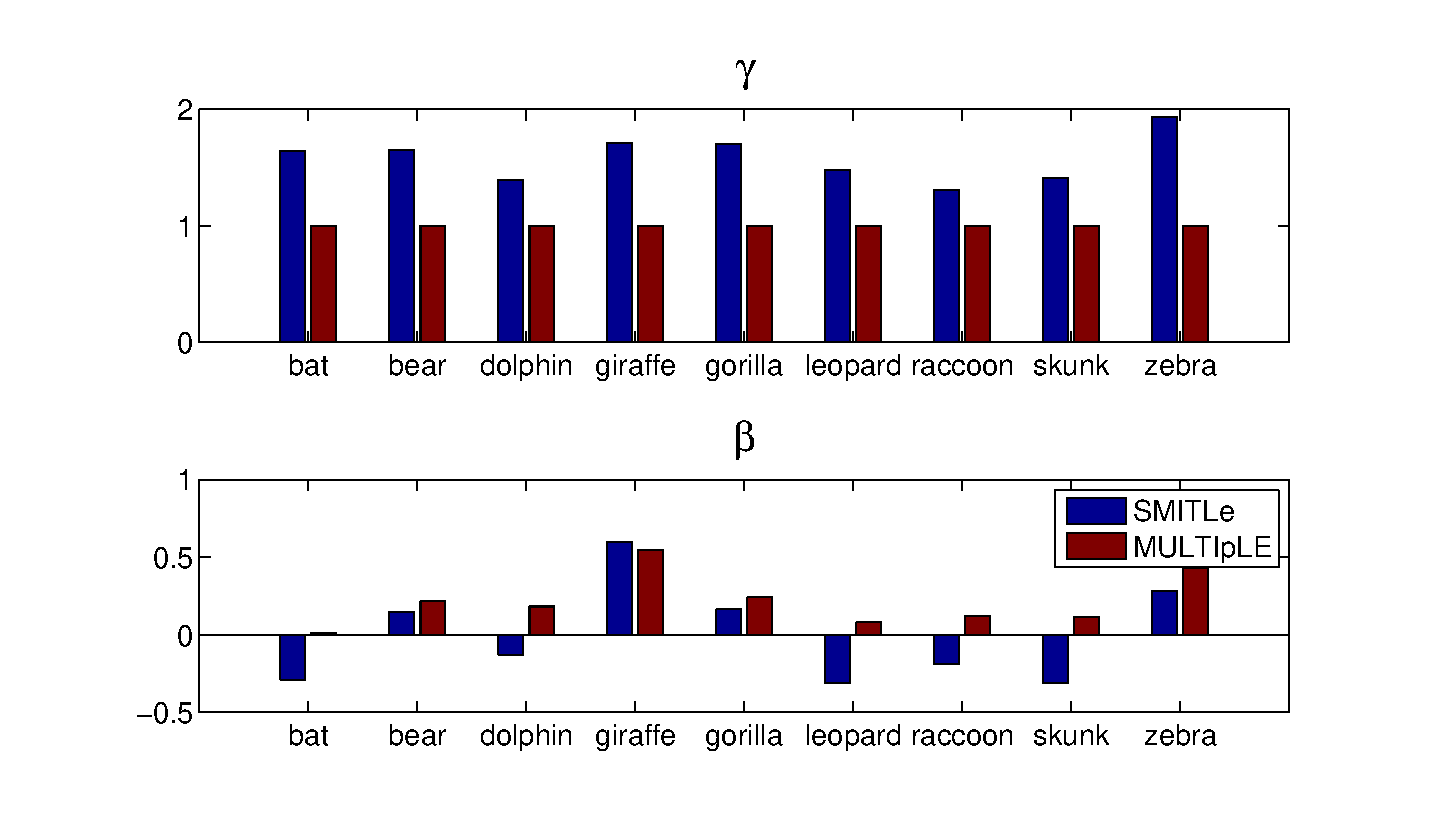
\includegraphics[scale=0.25]{fig/A2A_gama.eps} %\label{fig:awa-b}
\caption{Experiment results for 10 classes, AwA. Horse is used as the new category. We can see that SMITLe tends to more aggressively exploit the related prior knowledge.}
\label{fig:awa}
\end{figure}


\begin{table}[h]
  \centering
  \caption{Average accuracy in percentage across all categories from Caltech to Caltech with different size of the training set in target problem. 30 examples are randomly chosen from each class to train the source classifier and 30 examples from each class are chosen for the test. }
    \begin{tabular}{|c|c|c|c|c|}
    \hline
      \# per category    & 5     & 10    & 15    & 20 \\
    \hline
    No transfer &         27.33  &         31.53  &         35.73  &         38.47  \\
    Source+1    &         43.33  &         43.87   &         44.33  &         44.57   \\
    MKTL        &         38.89  &         43.27   &         45.72  &         47.44   \\
    MULTIKT     &         37.96  &         42.89   &         45.96  &         47.32  \\
    MULTIpLE    &         42.63  &         45.63   &         47.81  &         48.73 \\
    SMITLe        &         \textbf{43.53 }&         \textbf{46.45 } &         \textbf{48.25 } &         \textbf{49.15 } \\
        \hline
    Batch       &         43.77  &         44.73   &         46.67  &         48.00 \\
    \hline
    \end{tabular}%
  \label{tab:C2C}%
\end{table}%

% Table generated by Excel2LaTeX from sheet 'Sheet1'
\begin{table}[h]
  \centering
  \caption{Average accuracy in percentage across all categories from AwA to AwA with different size of the training set in target problem. 50 examples are randomly chosen from each class to train the source classifier and 200 examples from each class are chosen for test.}
    \begin{tabular}{|c|c|c|c|c|}
    \hline
     \# per category    & 5     & 10    & 15    & 20 \\
    \hline
    No transfer &         23.52  &         26.79  &         29.60  &         31.50  \\
    Source+1    &         \textbf{ 39.00 } &         \textbf{ 39.34 } &         39.62 &         39.74  \\
    MKTL        &         31.46  &         34.76  &         37.41  &         38.81  \\
    MULTIKT     &         29.86  &         32.86  &         35.22  &         36.33  \\
    MULTIpLE    &         37.80  &         38.81  &         39.80  &         40.47  \\
    SMITLe        &        37.83  &         { 39.31 } &         \textbf{ 40.37 } &         \textbf{41.09} \\
        \hline
    Batch       &         39.62  &         40.18  &         40.67  &         41.44  \\
    \hline
    \end{tabular}%
  \label{tab:A2A}%
\end{table}%

\subsection{Negative transfer: transferring from incorrect hypotheses}
In this section, we show how our method performs in transferring knowledge between two different datasets, from AwA dataset to Caltech dataset. Following the settings in the previous experiment, the source models are trained from AwA dataset and transferred to Caltech dataset. %We iteratively select one category as the new one, running multiple times to get the average results for all the algorithms. 
We show the average performance of each algorithm in Table \ref{tab:A2C}. We can see that negative transfer does happen when transferring the knowledge from AwA to Caltech for all the algorithms except for ours. From the performance of Source+1, we can see that applying the source hypotheses directly leads to poor performance. We can conclude that even though these two datasets share some categories, the data distribution of the feature representation for the same category is not consistent. 

Still we take the experiment where the horse is considered as the new category to see the detail performance of each algorithm. % and show it in Figure \ref{fig:awa} . 
From here we can see that, not surprisingly, the accuracy of SMITLe shows similar accuracy to the no transfer baseline, while other methods suffer from negative transfer and perform even worse than no transfer baseline. In Figure \ref{fig:a2c} we show the parameters learned for each classes in SMITLe in comparison with MULTIpLE. We can see that when the prior knowledge is unrelated, SMITLe resists utilizing the prior knowledge and, therefore, shows almost identical accuracy to the no transfer baseline.
%\begin{figure*}
%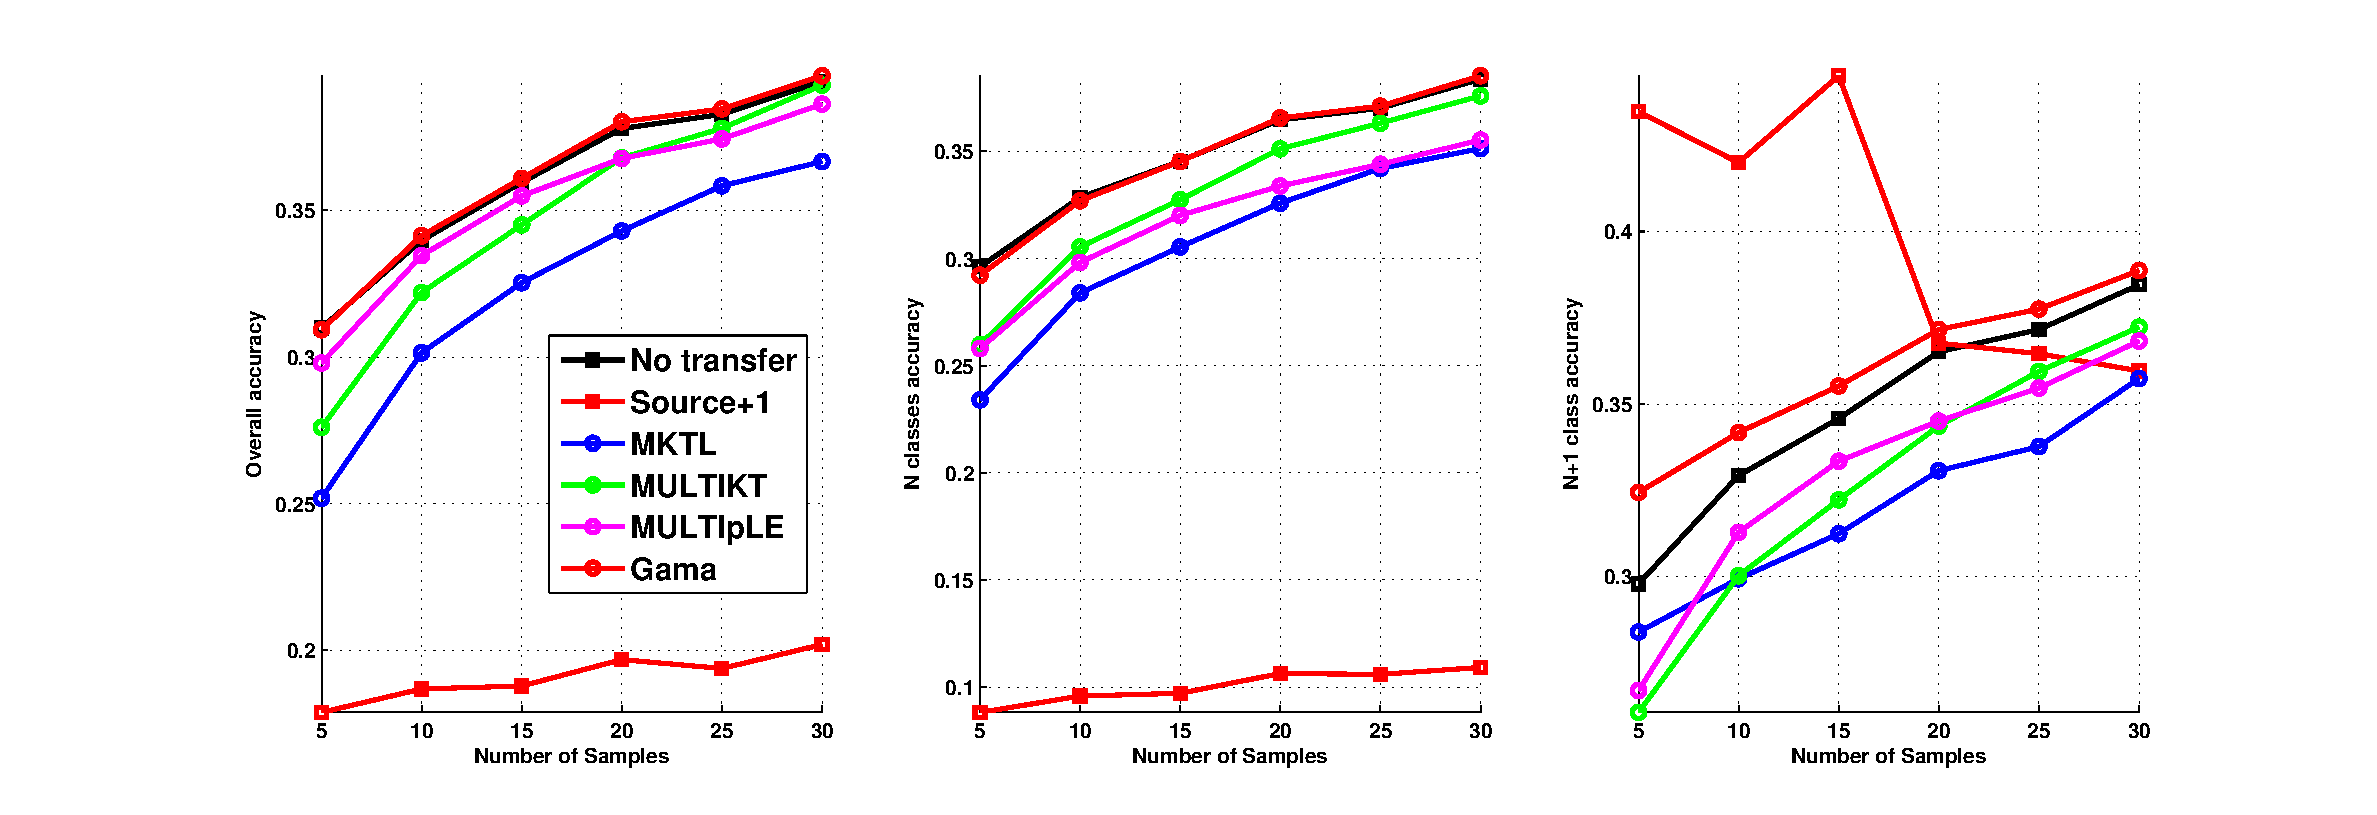
\includegraphics[width=\textwidth,height=5cm]{fig/A2C_RBF_PHOG.eps}
%\caption{Transferring from AwA to Caltech-256.}
%\end{figure*}
% Table generated by Excel2LaTeX from sheet 'Sheet1'

\begin{figure}
    \centering
     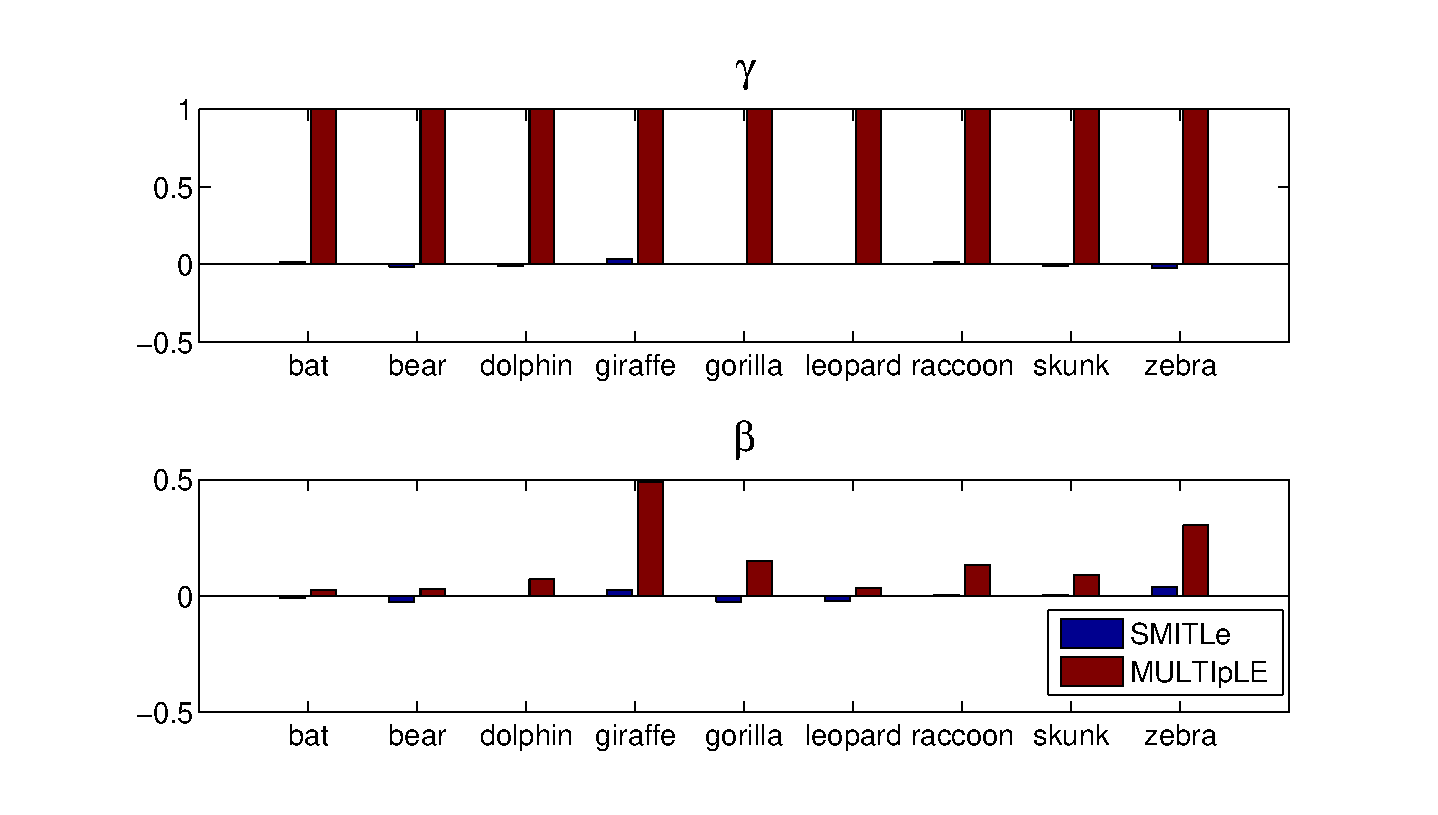
\includegraphics[scale=0.25]{fig/A2C_gama.eps} %\label{fig:a2c-b}
    \caption{Experiment results for 10 classes, AwA. Horse is used as the new category. SMITLe can ignore unrelated prior knowledge.}
    \label{fig:a2c}
\end{figure}


\begin{table}[htbp]
  \centering
  \caption{Average accuracy in percentage across all categories from AwA to Caltech. Examples in AwA are used to train prior models. Different number of training size is randomly selected from Caltech dataset.}
    \begin{tabular}{|c|c|c|c|c|c|}
    \hline
      \# per category           & 5              & 10             & 15             & 20             & 25             \\
    \hline
    No transfer &         \textbf{ 30.99 } &         33.97  &         35.95 &         37.78  &         38.27   \\
    Source+1    &         17.89  &         18.69  &         18.79  &         19.69  &         19.39          \\
    MKTL        &         25.19  &         30.14  &         32.53  &         34.30  &         35.83  \\
    MULTIKT     &         27.60  &         32.19  &         34.51  &         36.78  &         37.79  \\
    MULTIpLE    &         29.79  &         33.45  &         35.49  &         36.77  &         37.43  \\
    SMITLe        &       30.93  &         \textbf{ 34.13 } &         \textbf{  36.09 } &         \textbf{38.01} &         \textbf{38.46} \\
    \hline
    \end{tabular}%
  \label{tab:A2C}%
\end{table}%

\subsection{Transferring from mixed hypotheses}
In real applications, the extreme situation is rare. For most multi-source transfer learning tasks, there should always be some related and useful sources as well as some unrelated ones. In this part, we show how SMITLe performs in the mixed sources.

From negative transfer experiments we see that the knowledge from AwA is unrelated to Caltech and vice versa. To generate mixed sources, we follow the settings in our positive transfer experiment, splitting the AwA dataset into two datasets, and replace the data in some categories in the source dataset with the data of Caltech. 
For example, if the bat is considered as the new category and we have to replace 3 categories, we choose the data from 3 out of 9 categories (10 categories except for bat) in Caltech to replace the source data accordingly. 

We show the performances across all categories of different algorithms in Table \ref{tab:3c} and Table \ref{tab:4c} where 3 and 4 categories in the source data are replaced by the data from Caltech respectively. From the tables, we can see that in almost every case, SMITLe shows improved or equivalent performance than other baselines. %The improved performance of SMITLe is due to the loss function we designed. Compared to other transfer baselines, the loss function Eq. \eqref{eq:loss} is able to control the transfer parameters $\gamma$ and $\beta$ to prevent negative transfer. For other transfer baselines, such as Multi-KT and MULTIpLE, they try to optimize a convex function directly with non-negative L2 ball constraint, which could not be able to handle the negative transfer effectively.

% Table generated by Excel2LaTeX from sheet 'Sheet1'
\begin{table}[htbp]
  \centering
  \caption{Average accuracy in percentage across all categories from AwA to AwA\&Caltech with different size of the training set in target problem. Data of 3 classes in AwA is replaced by the data from Caltech in target problem.}
    \begin{tabular}{|c|c|c|c|c|c|}
    \hline
      \# per category    & 5     & 10    & 15    & 20    & 25 \\
    \hline
    no transfer &         23.99  &         26.24  &         29.02  &         30.05  &         31.18  \\
    source+1 &         25.70  &         26.30  &         26.57  &         26.69  &         26.97  \\
    MKTL  &         25.30  &         27.59  &         30.42  &         31.01  &         31.97  \\
    MultiKT &         25.53  &         27.94  &         30.48  &         31.36  &         32.31  \\
    MULTIpLE &         28.11  &         29.61  &         31.34  &         32.18  &         32.89  \\
    SMITLe &         \textbf{28.75}  &         \textbf{30.48}  &         \textbf{32.30}  &         \textbf{33.06}  &         \textbf{33.71}  \\
    \hline
    \end{tabular}%
  \label{tab:3c}%
\end{table}%



% Table generated by Excel2LaTeX from sheet 'Sheet1'
\begin{table}[htbp]
  \centering
  \caption{Average accuracy in percentage across all categories from AwA to AwA\&Caltech with different size of the training set in target problem. Data of 4 classes in AwA is replaced by the data from Caltech in target problem.}
    \begin{tabular}{|c|c|c|c|c|c|}
    \hline
       \# per category    & 5     & 10    & 15    & 20    & 25 \\
    \hline
    no transfer &         24.02  &         26.25  &         29.06  &         30.07  &         31.20  \\
    source+1 &         23.23  &         23.80  &         24.03  &         24.21  &         24.47  \\
    MKTL  &         24.44  &         26.78  &         29.64  &         30.40  &         31.50  \\
    MultiKT &         24.73  &         27.40  &         29.93  &         30.91  &         31.91  \\
    MULTIpLE &         26.50  &         28.33  &         30.27  &         31.29  &         32.12  \\
    SMITLe &         \textbf{27.20}  &         \textbf{29.33}  &         \textbf{31.40}  &         \textbf{32.31}  &         \textbf{33.11}  \\
    \hline
    \end{tabular}%
  \label{tab:4c}%
\end{table}%
